\documentclass[./main.tex]{subfiles}
\appendix               
\begin{document}      
%\addpart*{Appendix}             %% adding Appendix to tableofcontents
\chapter{Lagrange polynomial interpolation}
\label{chap:AppendixA}

\section{Introduction}

In this chapter, a short introduction to Lagrange polynomial interpolation is presented. This writeup is based on the NIST Library of Mathematical Functions $^{\cite{NIST}}$. \newline
The nodes $z_k$ are real or complex valued, the function values are $f_k = f(z_k)$.
Given $(n+1)$ distinct points $z_k$ with their corresponding function values $f_k$, the Lagrange interpolation polynomial is the unique polynomial $P_n(z)$ satisfying $P(z_k)=f_k$ while not exceeding order $n$, with $k = 0,1,...,n$. The Lagrange polynomial is given by

\begin{equation*}
	P_n(z) = \sum_{k=0}^{n} \mathscr{L}_k(z)f_k 
\end{equation*}

with Lagrange coefficients

\begin{equation*}
\mathscr{L}_k(z) =  \prod_{j=0, j \neq k}^{n} \frac{z-z_j}{z_k-z_j}
\end{equation*}

where the factor for $j=k$ is omitted in the product. The Lagrange coefficients are again polynomials with the property

\begin{equation*}
\mathscr{L}_k(z_j) =  \delta_{k,j},
\end{equation*}

thus, each $\mathscr{L}_k(z)$ has a weight of 1 if $z = z_k$ or 0 if $z = z_j$ with $j \ne k$. For this property, $P_n(z)$ goes exactly through all data points $(z_k,f_k)$. 

\section{Application for a simple exponential}
In practice one applies a low order polynomial interpolation for a small set of points lying close to the target position, this approach guarantees smoothness of the interpolated curve even for non-smooth data, thus effectively reducing high order polynomial oscillations.
For demonstrative purposes, some Lagrange polynomials (line style: solid, black) for a basic exponential function (line style: dotted, blue) are depicted below.


\begin{figure}[h!]
	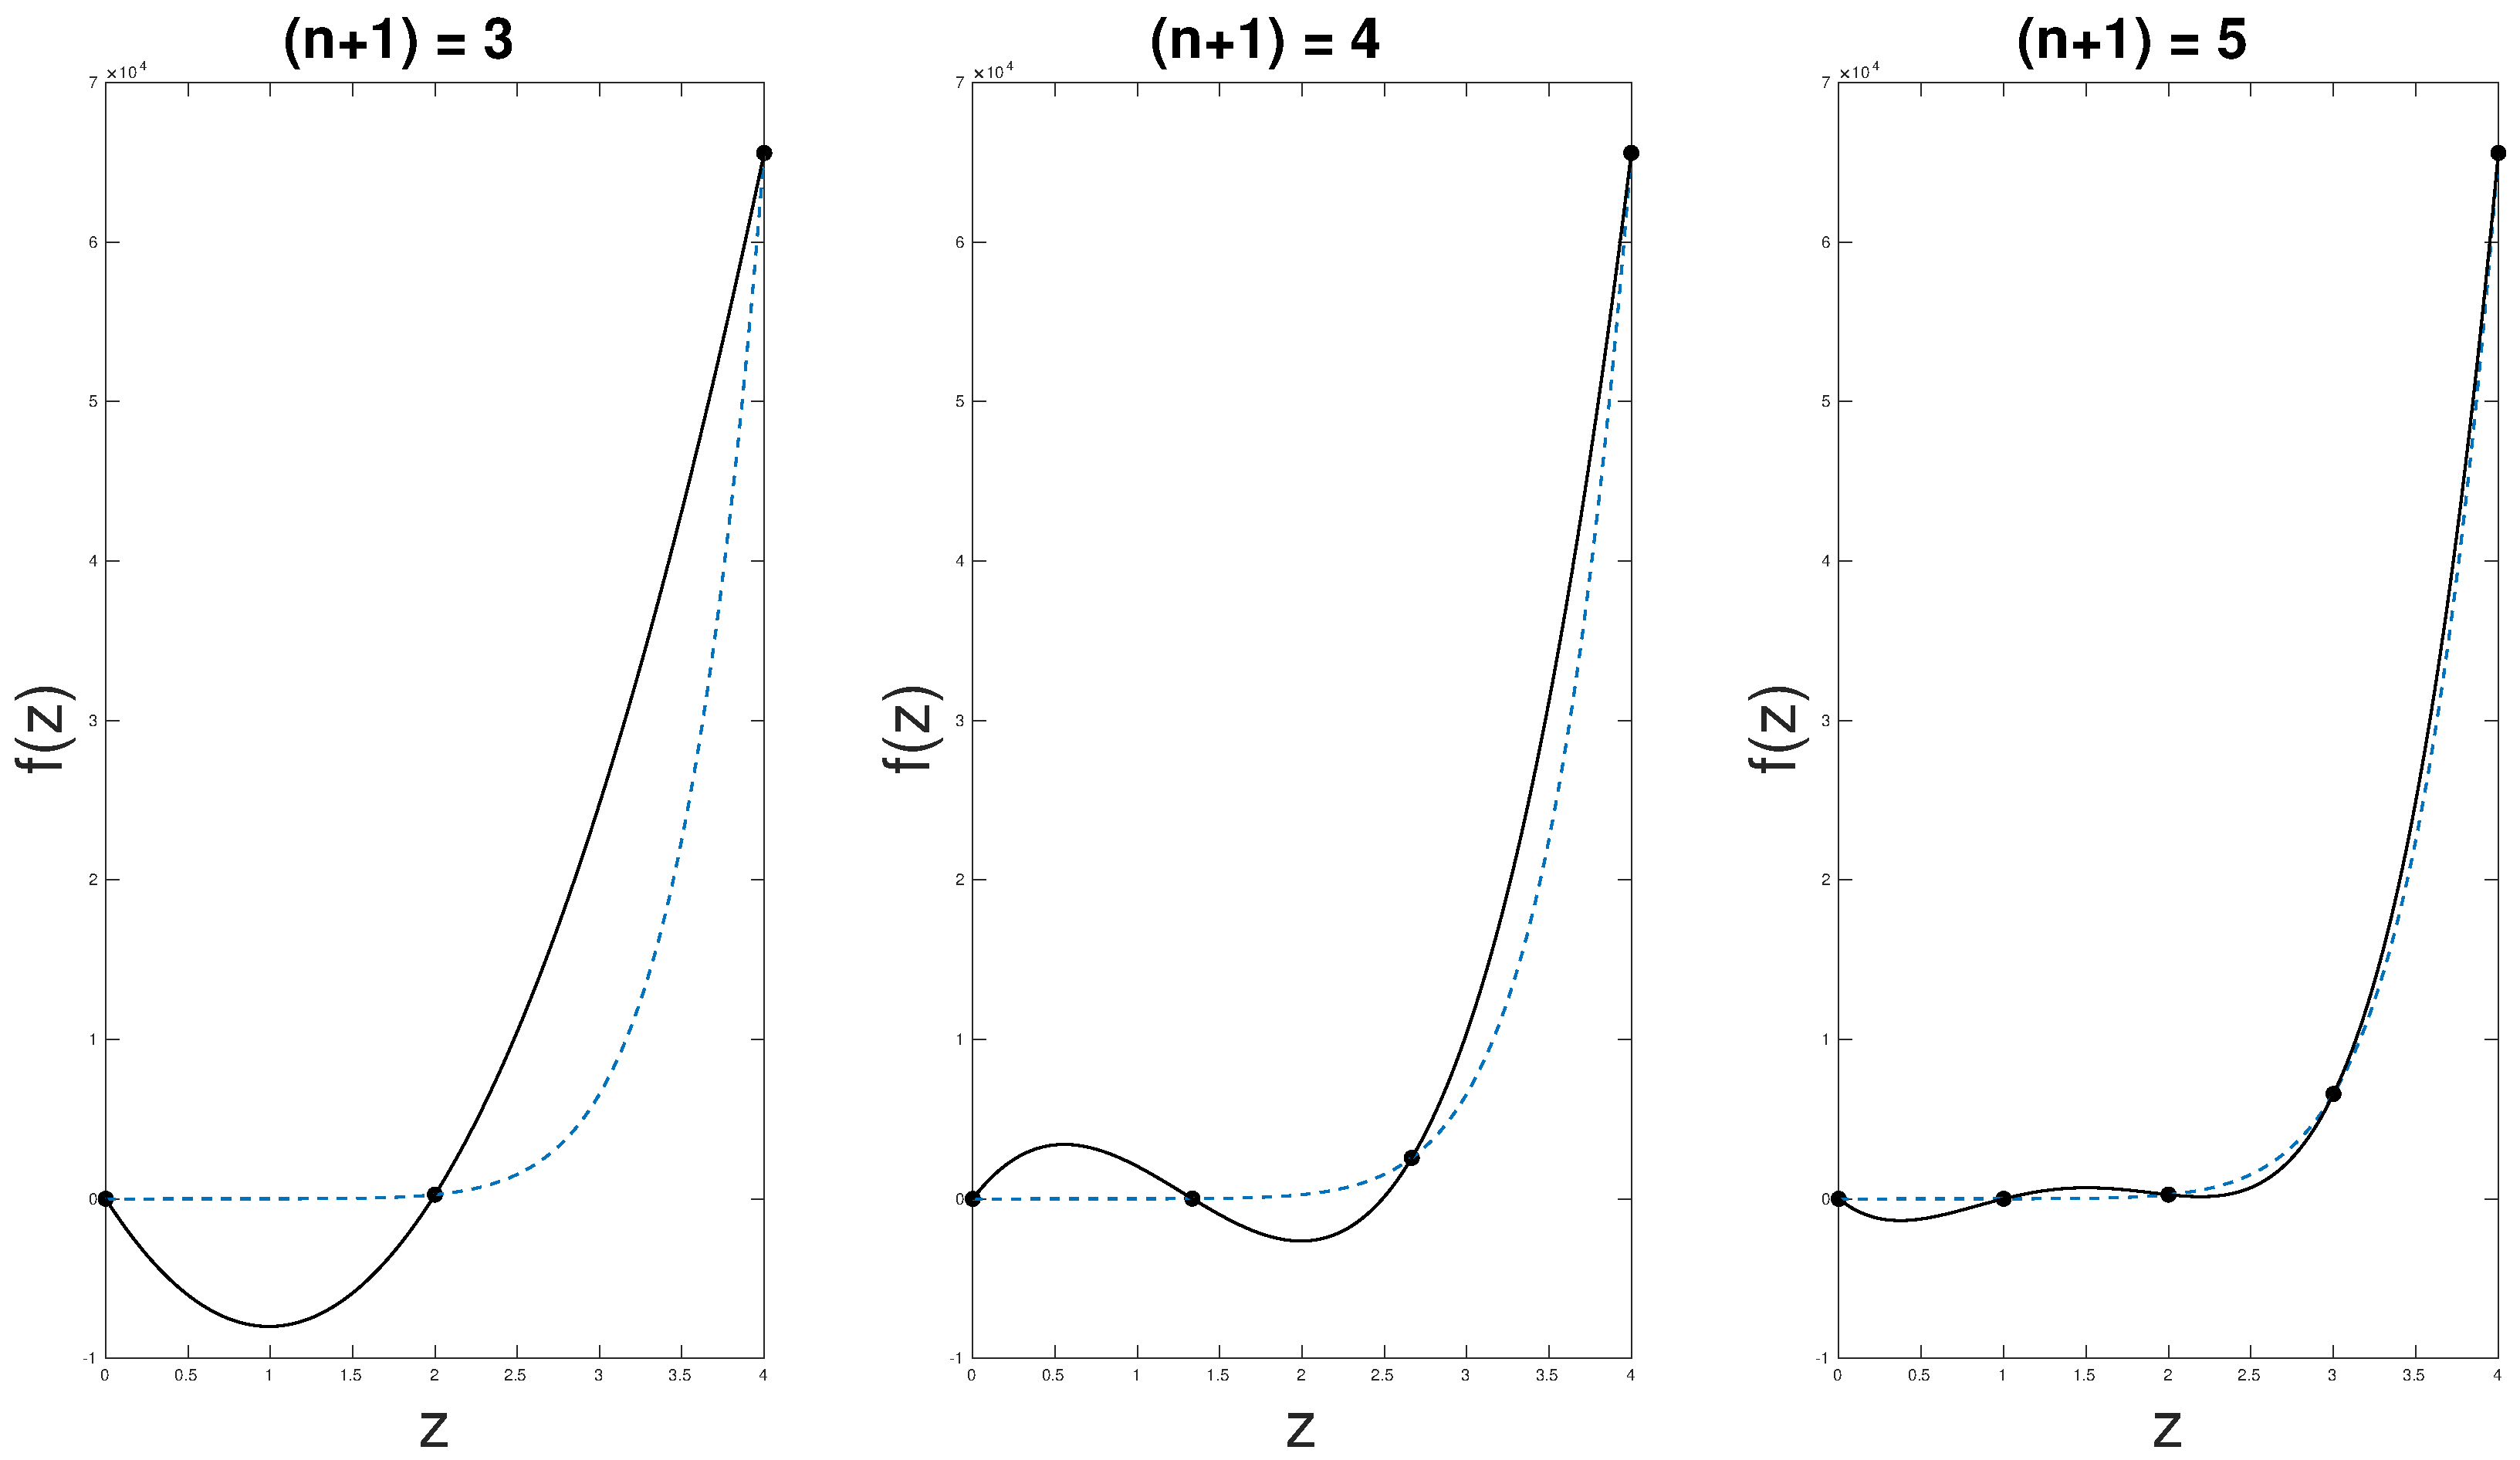
\includegraphics[width = 1.0\textwidth]{figures/lagrange_interp_plot1.eps}
	\caption{Lagrange polynomials of order $n$ with equidistant $z_k$ for $f(z) = e^z$}
	\label{lagrange_interp}
\end{figure}

%\section{Application for subroutine \texttt{theta\_geom2theta\_flux}}
%
%\begin{figure}[h!]
%	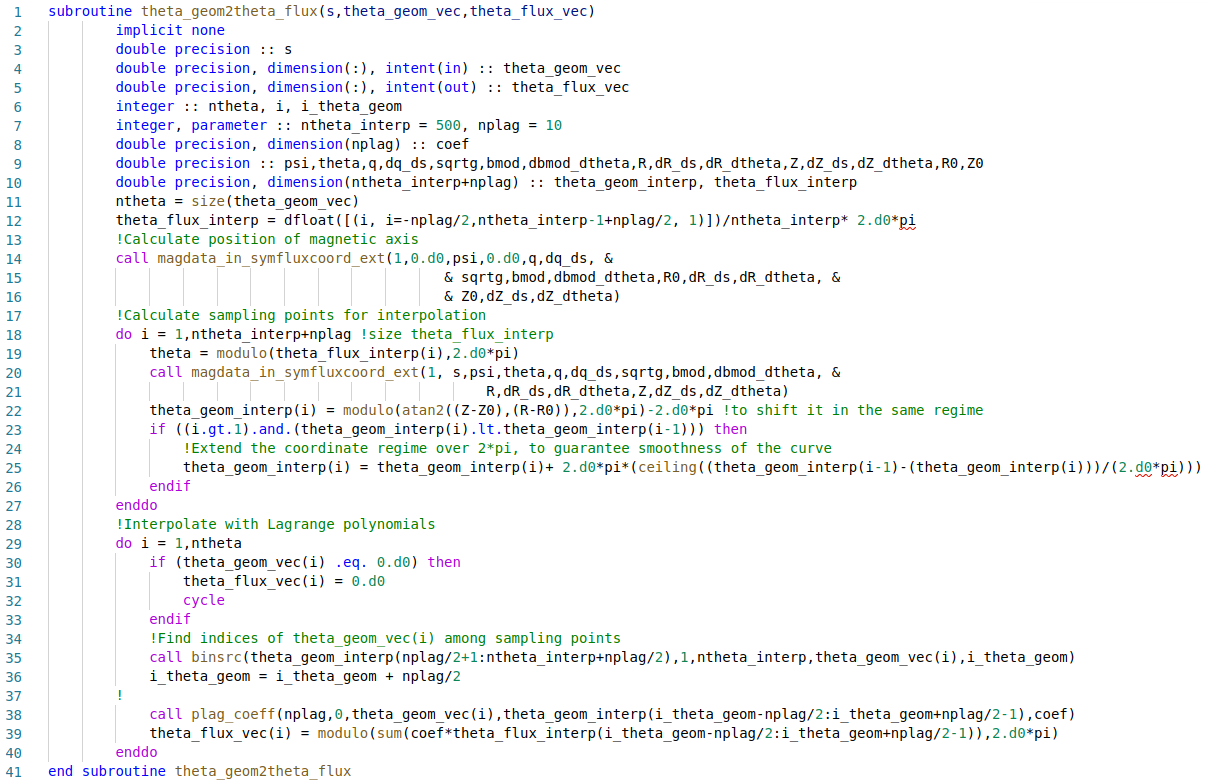
\includegraphics[width = 1.05\textwidth]{figures/theta_geom2theta_flux.png}
%	\caption{Fortran source code for subroutine \texttt{theta\_geom2theta\_flux}}
%	\label{lagrange_interp}
%\end{figure}


\newpage
\chapter{Runge-Kutta integration}
\label{chap:AppendixB}
\section{General formulation}
In this chapter, a brief summary of Runge-Kutta integration is presented, based on the comprehensive summary by E. Hairer in \cite{Hairer}. 
In numerical analysis, efficient integration methods for solving initial value problems of the form $y^\prime = f(x,y)$ were initially implemented by Euler (1768), although later further methods based on his work were developed by Runge (1895) and Kutta (1905). The most widely known algorithm is the so-called fourth order Runge-Kutta solver (commonly abbreviated \textit{RK4}), however, an entire generalized class of integrators has since been derived. Such an integrating scheme is fully described by the coefficients of the corresponding \textit{Butcher tableau} given in \ref{tab:Butcher_general}:

\begin{table}[h]
\caption{\textit{Butcher tableau} for a general \textit{s}-stage \textit{Runge-Kutta method}}
\label{tab:Butcher_general}
\[
\renewcommand\arraystretch{1.2}
\begin{array}
{c|ccccc}
0\\
c_2 & a_{21}\\
c_3 & a_{31} & a_{32} \\
\vdots& \vdots& \vdots& \ddots\\
c_s & a_{s1}& a_{s2} &\hdots& a_{s,s-1}\\
\hline
& b_1 &b_2 &\hdots &b_{s-1}&b_s\\ 
\end{array}
\]
\end{table}

Generally, the condition 

\be{eq:condition_coefficients_RK}
c_i = \sum^{i-1}_{j=1}a_{ij}
\ee

is further imposed, which greatly simplifies the problem of deriving order conditions for higher order methods.\\
Using the coefficients of \ref{tab:Butcher_general} one can explicitly calculate the approximate solution to the initial value problem for a single step $\Delta x = h$ by computing
\bea{eq:RK_y1}
\nonumber
y_1 &=& y_0 + h(b_1k_1+\hdots+b_sk_s)\\
\eea
with

\bea{eq:RK_general}
\nonumber
k_1 &=& f(x_0,y_0)\\
k_2 &=& f(x_0+c_2h,y_0+ha_{21}k_1)\\
\nonumber
k_3 &=& f(x_0+c_3h,y_0+h(a_{31}k_1+a_{32}k_2))\\
\nonumber
&\hdots\\
\nonumber
k_s &=&f(x_0+c_sh,y_0+h(a_{s1}k_1+\hdots+a_{s,s-1}k_{s-1})).\\
\nonumber
\eea
\section{RK4 with application}
For the specific case of the \textit{RK4}-method, which is also implemented in the \textit{GORILLA} code, the corresponding \textit{Butcher tableau} is given in \ref{tab:Butcher_RK4}. 

\begin{table}[h]
\caption{\textit{Butcher tableau} for the \textit{RK4}-method}
\label{tab:Butcher_RK4}
\[
\renewcommand\arraystretch{1.2}
\begin{array}
{c|cccc}
0\\
\frac{1}{2} & \frac{1}{2}\\
\frac{1}{2} &0 &\frac{1}{2} \\
1& 0& 0& 1\\
\hline
& \frac{1}{6} &\frac{1}{3} &\frac{1}{3} &\frac{1}{6} 
\end{array}
\]
\end{table}

One is especially interested in the application of this scheme to an ODE system of the shape

\be*{}
f(\tau,\mathbf{z}(\tau))= \mathbf{f}(\mathbf{z}(\tau)) =\frac{\textrm{d}\mathbf{z}(\tau)}{\textrm{d}\tau} = \hat{\mathbf{a}}\cdot\mathbf{z}(\tau) + \mathbf{b}\\
\ee 
with initial conditions $\mathbf{z}(0) = \mathbf{z}_0$. Note that $\mathbf{f}(\tau,\mathbf{z}(\tau))$ does not explicitly depend on $\tau$, thus, \eq{eq:RK_y1} and \eq{eq:RK_general} yield for a single \textit{RK4} step with $h = \tau$
\bea*{}
\nonumber
\mathbf{z}_{RK4} &=& \mathbf{z}_{0} + \tau \left( \frac{1}{3}k_1 + \frac{1}{6}k_2 + \frac{1}{6}k_3 + \frac{1}{3}k_4\right)\\
\nonumber
k_1 &=& \mathbf{f}(\mathbf{z}_{0})\\
k_2 &=& \mathbf{f}\left(\mathbf{z}_{0}+\frac{\tau}{2}\mathbf{f}(\mathbf{z}_{0})\right)\\
\nonumber
k_3 &=& \mathbf{f}\left(\mathbf{z}_{0}+\frac{\tau}{2}\mathbf{f}\left(\mathbf{z}_{0}+\frac{\tau}{2}\mathbf{f}(\mathbf{z}_{0})\right)\right)\\
\nonumber
k_4 &=& \mathbf{f}\left(\mathbf{z}_{0}+\tau \mathbf{f}\left(\mathbf{z}_{0}+\frac{\tau}{2}\mathbf{f}\left(\mathbf{z}_{0}+\frac{\tau}{2}\mathbf{f}(\mathbf{z}_{0})\right)\right)\right),\\
\nonumber
\eea
which allows to explicitly write the approximate \textit{RK4}-solution for this ODE system as 
\bea{}
\textbf{z}_{RK4}(\tau) &=& \textbf{z}_0 + \frac{\tau}{6}\textbf{f}(\textbf{z}_0)+\frac{\tau}{3}\textbf{f}\left(\textbf{z}_0 + \frac{\tau}{2}\textbf{f}(\textbf{z}_0)\right)
+\frac{\tau}{3}\textbf{f}\left(\textbf{z}_0 + \frac{\tau}{2}\textbf{f}\left(\textbf{z}_0 + \frac{\tau}{2}\textbf{f}(\textbf{z}_0)\right)\right)
\nonumber \\
&+&
\frac{\tau}{6}\textbf{f}\left(\textbf{z}_0 + \tau \textbf{f}\left(\textbf{z}_0 + \frac{\tau}{2}\textbf{f}\left(\textbf{z}_0 + \frac{\tau}{2}\textbf{f}(\textbf{z}_0)\right)\right)\right)~.
\eea

It is important to note that the \textit{RK4}-method has the property that for sufficiently smooth functions, the approximate \textit{RK4}-solution $\mathbf{z}_{RK4}(\tau)$ coincides with the fourth order Taylor expansion of the analytical solution for $\mathbf{z}(\tau)$. The associated errors are therefore of order $\mathcal{O}(\tau^5)$. \clearpage
\section{Runge-Kutta-Fehlberg - RK45}
Although the introduced \textit{RK4}-method is a very useful tool, its accuracy greatly depends on the chosen step size $h$, while the routine generally does not yield an estimate for the error, if not computed separately. A clever way to circumvent this problem was introduced by E. Fehlberg (1969), namely, to evaluate a given step successively with proposed fourth-order and fifth-order routines and then compute the difference of these two results. If the difference is smaller than a set tolerance, the step is accepted, if not, the step is discarded and the previous step size $h$ is halved for the next attempt.
The Butcher tableau for the \textit{RK45} method is given by \\

\begin{table}[h]
\caption{\textit{Butcher tableau} for the \textit{RK45}-method}
\label{tab:Butcher_RK45}
\[
\renewcommand\arraystretch{1.2}
\begin{array}
{c|ccccccc}
0\\
\frac{1}{4} & \frac{1}{4}\\
\frac{3}{8} & \frac{3}{32} &\frac{9}{32} \\
\frac{12}{13}& \frac{1932}{2197}& -\frac{7200}{2197}\\
1& \frac{439}{216}&-8&\frac{3680}{513}&-\frac{845}{4104} \\
\frac{1}{2}&-\frac{8}{27}&2&-\frac{3544}{2565}&\frac{1859}{4104}&-\frac{11}{40}\\
\hline
& \frac{16}{135}&0&\frac{6656}{12825}&\frac{28561}{56430}&-\frac{9}{50}&\frac{2}{55}\\
&\frac{25}{216}&0&\frac{1408}{2565}&\frac{2197}{4104}&-\frac{1}{5}&0\\
\end{array}
\]
\end{table}
Here, the first row at the bottom gives the coefficients for the fifth order method, the second row gives the coefficients for the fourth order method.

\end{document}